\documentclass{article}
\usepackage{amsmath,esint,textcomp,hyperref,graphicx,geometry,natbib,caption,subcaption,tikz}
\geometry{left=2.5cm,right=2.5cm,top=2.5cm,bottom=2.5cm}
\title{ \huge Semiconductor Solver \\
  \large Computational Physics (PH354) Project}
\author{Gaurav Somani}
\date{19 June 2020}
\hypersetup{
    colorlinks=true,
    linkcolor=blue,
    filecolor=magenta,      
    urlcolor=red,
}
\urlstyle{same}

\begin{document}
\maketitle
\pagenumbering{gobble}
\newpage
\pagenumbering{arabic}

\setcounter{section}{-1}
\section{Project Description}
\textbf{Semiconductor Solver (Equilibrium and steady state simulation)}:

This project solves Poisson's eqaution in 1D and 2D (with cylindrical and cartesian geometry) to calculate equilibrium potential inside semiconductor. Steady state solution calculation for 1D semiconductor is also implemented.                                                                                                                                      Both Maxwell-Boltzmann and Fermi-Dirac statistics are available for calculating equilibrium carrier population. Poisson equation with Maxwell-Boltzmann statistics is called Poisson-Boltzmann equation which is non-linear. So, there are no analytic solutions available for most devices (analytical solutions available are only for special 1D doping profiles and boundary conditions).                                                                                                                                                                                                                           Both potential(dirichlet) and potential derivative (Normal electric field) boundary conditions are considered. In most cases, boundary conditions should be consistent with charge conservation. Electric flux over the boundary of domain determines the charge within the domain. For charge neutrality, Electric flux over the boundary of domain should be 0. For 1D, this means same electric field at both ends of domain.  For 2D simulations, left and right bounadries have always reflecting boundary conditions. Top and bottom boundaries are set in input files.                                                                                                                                                                   For steady state solution poisson's equation along with electron and hole conservation equations are solved. SRH recombination-generation model is implemented with common lifetime for electrons and holes. In addition to SRH recombination, additional carrier generation can also be used by defining generation function in input file. Concept of quasi-fermi level along with Maxwell-Boltzman statistics is used to estimate non-equilibrium carrier distribution. Electric current, carrier population and potential profile are calculated. In addition to poisson's equation, two conservation equations (hole conservation and electron conservation) are used. Then, the three coupled equations relating potential,electron concentration and hole concentration are solved simultaneously.

For equilibrium, input file contains structure definition which contains mesh nodes with mesh spacing around nodes, boundary conditions on sections between nodes and a function which defines doping profile in the structure. Then, output of this structure definition (which is mesh and structure parameters) are set as input to the solve function. For steady state calculations, only 1D structures are allowed. First, the structure of interest needs to solved at equilibrium. Then, solution output should be loaded as input to steady state solver along with specifying biasing conditions at contacts.

Defaults material is Silicon and constants for Silicon are entered in \textbf{constants.py}.

Sample input files \verb!input_equlibrium_1d.py, input_equlibrium_2d.py, input_bias.py! are included in this repository. See them to understand how to write input files. Sample files can be run to regenerate documented results. Source code can be found in \textbf{src} folder


\section{Mathematical Formualtion}
\subsection{Thermal Equilibrium}
Thermal equilibrium implies that fermi level in the semiconductor remains constant through out the semiconductor (and equal to its surroundings) .The carriers inside the semiconductor are in equilibrium with surroundings and there is no net movement of carriers in any direction. This implies there is no net electron current and hole current in the device. 

So, the electrostatic potential inside semiconductor is given by Poisson equation. 

\begin{align*}
\nabla^2 \psi = -\frac{\rho}{\epsilon}\\
\rho = q(N_D - N_A + p - n)
\end{align*}

\begin{equation}
\nabla^2 \psi = -\frac{q(N_D - N_A + p - n)}{\epsilon} \tag{1.1} \label{eq:1}
\end{equation} 
where $\psi$ represents electrostatic potential and $q$ represents charge of electron, $\rho$ represents charge density and $\epsilon$ represents dielectric permittivity of semiconductor, $N_D$ represents the number of dopants, $N_A$ represents the acceptor density, $p$ represent hole density,$n$ represent electron density

Net doping ($N$) can be defined as difference of donor and acceptor density ($N_D-N_A$). So, \eqref{eq:1} can be rewritten as 

\begin{equation}
\nabla^2 \psi = -\frac{q(N + p - n)}{\epsilon} \tag{1.2}\label{eq:2}
\end{equation}\\

Electron and hole density are dependent on fermi level and band structure of semiconductor and given by Fermi-Dirac statistics. Complete Fermi-Dirac integral is used to calculate carrier density and its derivatives.\\

Complete Fermi-Dirac integral ($F_j$) is defined by

\begin{equation}
  F_j(x) = \frac{1}{\Gamma(j+1)}\int^\infty_0 \frac{t^j}{e^{t-x}+1} dt \tag{1.3} \label{eq:3}
\end{equation} 

It can be seen that $F_j(x) \approx e^x$ when $x << 0$. This approximation is valid if fermi level is not very close to band edges.

$n_i$ and $\psi_i$ are defined as
\begin{align*}
 n_i = \sqrt{N_C N_V} \frac{-E_g}{2k_BT}\\
 \psi_i = \frac{1}{2q}(E_g + k_B T\ ln\frac{N_C}{N_V}) \tag{1.4} \label{eq:4}  
\end{align*}

\begin{align*}
n = N_C F_{1/2}\left(\frac{q(\psi-\psi_i)}{k_BT}\right) \\
p = N_V F_{1/2}\left(\frac{-q(E_g+\psi-\psi_i)}{k_BT}\right) \tag{1.5} \label{eq:5}
\end{align*}
where $E_g$ is potential band gap of semiconductor, $N_C$ and $N_V$ represent effective density of states in conduction and valence band respectively. 

Using \eqref{eq:2} and \eqref{eq:5},

\begin{equation}
\nabla^2 \psi = -\frac{q}{\epsilon}(N + N_V F_{1/2}(\frac{-q(E_g+\psi-\psi_i)}{k_BT}) - N_C F_{1/2}(\frac{q(\psi-\psi_i)}{k_BT}))   \tag{1.6} \label{eq:6}
\end{equation}\\

In semiconductor devices, doping profiles and boundary conditions are cylindrically symmetric about vertical direction or uniform along one horizontal direction. Hence, electrostatic potential($\phi$) is also cylindrically symmetric about vertical direction or uniform along one horizontal direction 

For cylindrically symmetric $\phi$,
\begin{equation}
\nabla^2 \psi = \frac{\partial^2\phi}{\partial x^2} + \frac{1}{x}\frac{\partial\phi}{\partial x} + \frac{\partial^2\phi}{\partial y^2}  \tag{1.7} \label{eq:7}
\end{equation}
where $x$ represents radial distance and $y$ represents distance along cylindrical axis

For $\phi$ being uniform along one direction
\begin{equation}
\nabla^2 \psi = \frac{\partial^2\psi}{\partial x^2} + \frac{\partial^2\phi}{\partial y^2}   \tag{1.8} \label{eq:8}
\end{equation}
where $x$ represents horizontal axis and $y$ represents vertical axis

Here, in all cases, system is symmetric about left vertical axis (x=0).

In some cases, semiconductor has doping and boundary conditions variation along only one dimension. Then,$\phi$ varies only along one direction. Then, $\nabla^2 \phi$ becomes second derivative. 
\begin{equation}
\nabla^2 \psi = \frac{d^2\psi}{dy^2}  \tag{1.9} \label{eq:9}
\end{equation}
where $y$ represents dimension along which $\phi$ varies.

For cases with 1-D structure due to symmetry,
\begin{align*}
	\nabla^2 \psi = \frac{1}{x^n} \frac{d}{dx}\left( x^n\frac{d\phi}{dx} \right)
\end{align*}

where $x$ represents radial dimension, $n=1$ for cylindrical symmetry and $n=2$ for spherical symmetry 

\subsection{Steady State (Biased) Current flow}

In steady state, carriers flow in semiconductor but there density in the semiconductor does not vary with time.
So, along with the Poisson equation \eqref{eq:3}, hole conservation equation and electron conservation equation needs to be solved.

In semiconductor, while carriers move, carriers can recombine which leads to reduction in carrier population. For conservation of electrons and holes, carriers need to be injected into the device. This leads to conservation equations which relate recombination rate to carrier current density.

Recombination rate is rate at which carriers combine per unit volume per unit time.

\begin{equation}
R =  \frac{\vec{\nabla}.\vec{J_n}}{q} =-\frac{\vec{\nabla}.\vec{J_p}}{q}   \tag{1.10} \label{eq:10}
\end{equation}

Since semiconductor is not in thermal equilibrium, there is no notion of fermi level. So, carrier density is no longer given by \eqref{eq:4} and \eqref{eq:5}. Also, now we have 3 equations (\eqref{eq:2} and \eqref{eq:11}). But the unknowns are $\psi$, $n$, $p$, $\vec{J_p}$, $\vec{J_n}$ and $R$. 3 more equations are required to solve the problem.\\

Most common is drift-diffusion formulation used to obtain carrier current densities.

\begin{align*}
\vec{J_n} = -qn\mu_n\nabla\phi_n \\ 
\vec{J_p} = -qp\mu_p\nabla\phi_p  \tag{1.11} \label{eq:11}
\end{align*}

where $\mu_n$ and $\mu_p$ represent electron and hole mobility respectively and $\phi_n$ and $\phi_p$ represent electron and hole quasi-fermi level respectively.

Total current density is given by
\begin{align*}
\vec{J} = \vec{J_n} + \vec{J_p}
\end{align*}

To obtain electron and hole densities with given quasi-fermi levels, $F_j(x) \approx e^x$ is used(in most cases, quasi-fermi level is far from band edge). 

\begin{align*}
n = n_i\ exp({\frac{q(\psi-\phi_n)}{k_BT}}) \\
p = n_i\ exp({\frac{-q(\psi-\phi_p)}{k_BT}}) \tag{1.12} \label{eq:12}
\end{align*}

Along with this, SRH model for recombination leads to
\begin{equation}
R = \frac{pn - n_i^2}{\tau_n(p + n_i) + \tau_p(n + n_i)} \tag{1.13}\label{eq:13}
\end{equation}

where $n_i$ represents equilibrium carrier concentration given by \eqref{eq:4} and $\tau_n$ and $\tau_p$ are electron and hole lifetimes respectively.

Additional generation mechanism can be added to this.   
\eqref{eq:10} cam be rewritten as 

\begin{equation}
R - G =  \frac{\vec{\nabla}.\vec{J_n}}{q} =-\frac{\vec{\nabla}.\vec{J_p}}{q}   \tag{1.14} \label{eq:38}
\end{equation}

where $G$ is additional generation due to some other physical process.

\subsection{Small Signal AC Current flow}
More generally, (when system is not in steady state), charge carrier density varies with time.

\begin{equation}
R - G = -\frac{\partial{n}}{\partial t} + \frac{\vec{\nabla}.\vec{J_n}}{q} = -\frac{\partial{p}}{\partial t} -\frac{\vec{\nabla}.\vec{J_p}}{q}   \tag{1.15} \label{eq:39}
\end{equation}

Consider a small variation over steady state variation with radial frequency $\omega$. Then,

\begin{align*}
\phi_n = ({\phi_n})_{dc} + ({\phi_n})_{ac}\ e^{\iota \omega t} \\
\phi_p = ({\phi_p})_{dc} + ({\phi_p})_{ac}\ e^{\iota \omega t} \\
\psi = \psi_{dc} + \psi_{ac} e^{\iota \omega t}
\end{align*}

where ${\phi_n}_{ac}$, ${\phi_p}_{ac}$ and $\psi_{ac}$ are are complex functions of space and represent the complex amplitudes of small signal fluctuations over steady state solution.

Let $F(\psi,\phi_n,\phi_p,\omega)$ be a function of $\psi$, $\phi_n$, $\phi_p$ and $\omega$. Then, $F$ is given by
\begin{align*}
F = F_{dc} + e^{\iota \omega t} \left({\frac{\partial F}{\partial \psi} \psi_{ac}+ \frac{\partial F}{\partial \phi_n} ({\phi_n})_{ac} +\frac{\partial F}{\partial \phi_p}({\phi_p})_{ac}}\right)_{\psi=\psi_{dc},\phi_n=({\phi_n})_{dc},\phi_p = ({\phi_p})_{dc},\omega=0} \\
where\ F_{dc} = F_{\psi=\psi_{dc},\phi_n=({\phi_n})_{dc},\phi_p = ({\phi_p})_{dc},\omega=0} 
\end{align*}

\begin{align*}
\implies \frac{\partial F}{\partial t} = \iota \omega e^{\iota \omega t} \left({\frac{\partial F}{\partial \psi} \psi_{ac}+ \frac{\partial F}{\partial \phi_n} ({\phi_n})_{ac} +\frac{\partial F}{\partial \phi_p}({\phi_p})_{ac}}\right)_{\psi=\psi_{dc},\phi_n=({\phi_n})_{dc},\phi_p = ({\phi_p})_{dc},\omega=0}
\end{align*}

\begin{align*}
\implies
F_{ac} = \left({\frac{\partial F}{\partial \psi} \psi_{ac}+ \frac{\partial F}{\partial \phi_n} ({\phi_n})_{ac} +\frac{\partial F}{\partial \phi_p}({\phi_p})_{ac}}\right)_{\psi=\psi_{dc},\phi_n=({\phi_n})_{dc},\phi_p = ({\phi_p})_{dc},\omega=0} \\
\left({\frac{\partial F}{\partial t}}\right)_{ac} = \iota \omega F_{ac}
\tag{1.16} \label{eq:ac_derivative}
\end{align*}

$\omega=0$ represents steady state solution.

Using the above relations, ac small signal amplitudes for charge carrier flux, recombination and carrier current density can be written for given steady state solution and $\omega$.

Since the carrier current density is changing with time, displacement current needs to be added to carrier current density such that total current density flux is zero.

For uniform $\epsilon$ (single semiconductor), displacement current density is given by
\begin{align*}
\vec{J_d} = \epsilon \frac{\partial \vec{E}}{\partial t}
\end{align*}
where
\begin{align*}
\vec{E} = -\nabla{\psi} 
\end{align*}

For one dimensional semiconductor, 
\begin{align*}
\vec{E} = -\nabla{\psi} = -\frac{\partial{\psi}}{\partial x} \hat{x} 
\end{align*}

Total current density is given by
\begin{align*}
\vec{J} = \vec{J_n} + \vec{J_p} + \vec{J_d}
\end{align*}

\subsection{Boundary Conditions}

Under thermal equilibrium, at each point on boundary, either electrostatic potential or electric field normal to the surface needs to specified at the boundary. For consistent boundary conditions, Electric flux should satisfy gauss law for given net charge inside semiconductor. 
\begin{equation}
   \varoiint \vec{E}.\vec{dS} =  \frac{1}{\epsilon} (net\ charge) = \frac{1}{\epsilon} \iiint \rho\ dV \tag{1.17} \label{eq:14}
\end{equation}

Since semiconductors are grown vertically,there is no electric field on horizontal boundaries of system as there is no electric charge present at both horizontal boundaries. Also, in all cases, system is symmetric about left vertical axis (x=0). So, left boundary is always reflecting.

For cylindrically symmetric $\phi$,
\begin{equation}
\int ((E_y)_{bottom} - (E_y)_{top})\ x \ dx  = \frac{1}{\epsilon} \iint \rho x\ dx\ dy \tag{1.18}\label{eq:15}
\end{equation}
where $x$ represents radial distance and $y$ represents distance along cylindrical axis

For $\phi$ being uniform along one direction
\begin{equation}
\int ((E_y)_{bottom} - (E_y)_{top}) \ dx  = \frac{1}{\epsilon} \iint \rho\ dx\ dy \tag{1.19}\label{eq:16}
\end{equation}
where $x$ represents horizontal axis and $y$ represents vertical axis

For one-dimensional semiconductor, 
\begin{equation}
(E_y)_{bottom} - (E_y)_{top}  = \frac{1}{\epsilon} \iint \rho\ dy \tag{1.20}\label{eq:17}
\end{equation}

For neutral semiconductors, this means electric flux over the boundary is zero. 
\begin{align*}	
   \oiint \vec{E}.\vec{dS} =  0
\end{align*}
\begin{align*}   
\int ((E_y)_{bottom} - (E_y)_{top})\ x \ dx  = 0\ for\ cylindrically\ symmetric\ \phi \\
\int ((E_y)_{bottom} - (E_y)_{top}) \ dx  = 0\ for\ \phi\ being\ uniform\ along\ one\ direction \\
(E_y)_{bottom} - (E_y)_{top}  = 0\ for\ one-dimensional\ semiconductor
   \tag{1.21} \label{eq:18}
\end{align*}

For specifying potential boundary conditions, ohmic and schottky contacts are possible. 
Under thermal equilibrium, schottky contacts specify a certain fixed potential at the boundary in addition to 
\begin{equation}
   \psi = \psi_i - \phi_B \tag{1.21} \label{eq:19}
\end{equation}
where $\phi_B$ represents schottky barrier 

Ohmic boundary condition is special type of boundary condition which imply there is no charge at the boundary point under thermal equilibrium. 

Under steady state current flow, ohmic contacts imply simple dirichlet boundary conditions, where surface
potential, electron density and hole density are fixed.
At boundary (under Maxwell-Boltzmann approximation),
\begin{align*}
\phi_n = \phi_p = V_{bias} \\
n = \frac{1}{2}({N + \sqrt{N^2 + 4n_i^2}}) \\
p = \frac{n_i^2}{n} \\ 
\psi = V_{bias} + \frac{k_BT}{q} ln\frac{n}{n_i} \tag{1.22} \label{eq:20}
\end{align*}

For small signal ac current in one dimensional semiconductor, since the equations are linearised with respect to ac values, the solution variables($\psi_{ac}$, $(\phi_n)_{ac}$ and $(\phi_p)_{ac}$) are set to 1 unit at one end and 0 at the other end.

Then, the small signal ac current density in the semiconductor is simply the admittance of device in chosen units.

\section{Numerical Formualtion}
\subsection{Normalisation}
Normalisation of equations reduces the original equation with physical units into dimensionless units.
\begin{align*}
V_T = \frac{k_BT}{q} \\ 
L_D = \sqrt{\frac{\epsilon V_T}{q n_i}} \\
E_0 = \frac{V_T}{L_D} \\
J_o = \frac{q \mu_n n_i V_T}{L_D} \\
t_0 = \frac{\epsilon}{q \mu_n n_i} \\
R_o = \frac{n_i}{t_0}
\tag{2.1} \label{eq:21} 
\end{align*}
$N_C$, $N_V$, $N$, $p$, $n$ and $n_i$ have units of doping density. $E_g$, $\psi$, $\phi_n$, $\phi_p$ and $V_T$  have units of potential. $L_D$ has dimensions of length.$E_0$ and $\vec{E}$ have dimensions of electric field.
$\vec{J_n}$, $\vec{J_p}$ and $J_o$ has dimensions of current density. $\mu_n$ and $\mu_p$ has dimensions of mobility. $G$,$R$ and $R_o$ has dimensions of recombination rate. $t_0$ and $\tau$ have dimensions of time.\\
Quantities with units of length, potential, electric field, dopant density, current density,\ recombination rate, time and mobility are scaled down by $L_D$, $V_T$, $E_0$, $n_i$, $t_n$, $J_o$, $R_o$, $t_0$ and $\mu_n$ respectively. 

For simplicity, notation remains the same but quantities refer to dimensionless quantities in the remaining sections unless otherwise stated. Normalised equations take the following form.
\begin{equation}
\nabla^2 \psi = n - p - N  \tag{2.2} \label{eq:22}
\end{equation}

\textbf{Equilibrium}:
Under equilibrium,
\begin{align*}
n =  N_C F_{1/2}(\psi-\psi_i) \\
p = N_V F_{1/2}(\psi_i-E_g-\psi)
\tag{2.3} \label{eq:23}
\end{align*}

\textbf{Steady state current flow}:
Under steady state current flow,
\begin{align*}
n = e^{\psi-\phi_n} \\
p = e^{-(\psi-\phi_p)} \\
R - G = \vec{\nabla}.\vec{J_n} = -\vec{\nabla}.\vec{J_p} \\
\vec{J_n} = -n\nabla\phi_n = -n\nabla\psi + \nabla n = n\vec{E} + \nabla n \\
\vec{J_p} = -p\mu_p\nabla\phi_p  = -p\mu_p\nabla\psi - \mu_p\nabla p = p\mu_p\vec{E} - \mu_p\nabla p \\
R = \frac{pn-1}{\tau_p(n+1) + \tau_n(p+1)}
\tag{2.4} \label{eq:24}
\end{align*}

Integral form of conservation equation can be written as
\begin{align*}
\iiint (R-G) dV = \varoiint \vec{J_n}.\vec{dS} = - \varoiint \vec{J_p}.\vec{dS} \\
For\ 1-D\ semiconductor,
\int (R-G)\ dx = \int J_n\ dx = - \int J_p\ dx \\
J_n = \frac{dn}{dx} + n E = -n \frac{d\phi_n}{dx}\\
J_p = -\mu_p\frac{dp}{dx} + p\mu_p E = -p \frac{d\phi_p}{dx}
\tag{2.5} \label{eq:25}
\end{align*}

\subsection{Linearisation}
Since Poisson equation along with fermi-dirac statistics for charge carriers is non-linear PDE, it needs to be linearised to make solution methods of linear algebra applicable.

Let $\Theta$ be a small deviation of the true solution of Poisson’s equation $\Phi$ from the approximate solution $\bar{\Phi}$. 
\begin{align*}
\Phi = \bar{\Phi} + \Theta \\
\implies \nabla^2 (\bar{\Phi} + \Theta) = \nabla^2 \bar{\Phi} + \nabla^2\Theta = n - p - N
\end{align*}

Since electron and hole densities depend on electrostatic potential, they will also deviate from true densities and this deviation can be linearised to linearise the equation. 
\begin{align*}
p \approx \bar{p} + \Theta\left(\frac{\partial p}{\partial \psi}\right)_{\psi = \bar{\Phi}} \\
n \approx \bar{n} + \Theta\left(\frac{\partial n}{\partial \psi}\right)_{\psi = \bar{\Phi}}  \\
\ where\ \bar{p} = p(\psi = \bar{\Phi})\ and\ \bar{n} =n(\psi = \bar{\Phi})
\end{align*}

\begin{equation}
\implies \nabla^2 \Theta = r + \Theta \left(\left(\frac{\partial n}{\partial \psi}\right)_{\psi = \bar{\Phi}} - \left(\frac{\partial p}{\partial \psi}\right)_{\psi = \bar{\Phi}}\right) \tag{2.6} \label{eq:26}
\ where\ r = (\bar{n} - \bar{p} - N) - \nabla^2 \bar{\Phi}
\end{equation}

\begin{align*}
  \frac{d}{dx}F_j(x) = F_{j-1}(x) \\
  \implies \frac{d}{dx} F_{1/2}(x) = F_{-1/2}(x) \tag{2.7} \label{eq:27}
\end{align*} 

\textbf{Equilibrium}:
Using \eqref{eq:23} and \eqref{eq:27}),
\begin{align*}
\frac{\partial n}{\partial \psi} =  N_C F_{-1/2}(\psi-\psi_i) \\
\frac{\partial p}{\partial \psi} = -N_V F_{-1/2}(\psi_i-E_g-\psi) \tag{2.8} \label{eq:28}
\end{align*} 

Using \eqref{eq:26} and \eqref{eq:28},
\begin{align*}
\nabla^2 \Theta = r + \Theta ( N_C F_{-1/2}(\bar{\Phi}-\psi_i) + N_V F_{-1/2}(\psi_i-E_g-\bar{\Phi})) \tag{2.9} \label{eq:29}
\end{align*} 

\textbf{Steady state current flow}:
\begin{align*}
\frac{\partial n}{\partial \psi} = e^{\psi-\phi_n} = n \\
\frac{\partial p}{\partial \psi} = -e^{-(\psi-\phi_p)} = -p \\
\frac{\partial n}{\partial \phi_n} = -n \\
\frac{\partial p}{\partial \phi_p} = p 
\tag{2.10} \label{eq:30}
\end{align*} 

At steady state with quasi fermi levels (using \eqref{eq:24} ),
\begin{align*}
\nabla^2 \Theta = r + \Theta ( e^{\bar{\Phi}-\phi_n} + e^{-(\bar{\Phi}-\phi_p)}) \tag{2.11} \label{eq:31}
\end{align*} 

Continuity equations need to be linearised with respect to $d\phi_n$, $d\phi_p$ and $d\psi$ where $d(variable)$ implies the correction in the solution to approximate solution in current iteration. In following equations, $\bar{s}$ represents the approximate solution $s$ from previous iteration (value of variable about which the variable is linearised). Charge carrier flux and recombination needs to be linearised.

In discretisation of charge carriers flux, $\alpha$ and $\beta$ are defined.

\begin{align*}
\alpha = e^{-\phi_n}  \\
\beta = e^{\phi_p}
\end{align*}

\begin{align*}
\phi_n = \bar{\phi_n} + d\phi_n   \\
\phi_p = \bar{\phi_p} + d\phi_p 
\end{align*}

\begin{align*}
\implies \alpha = e^{-(\bar{\phi_n} + d\phi_n)} = e^{-\bar{\phi_n}} (1 - d\phi_n)  \\
\beta = e^{\bar{\phi_p} + d\phi_p} = e^{\bar{\phi_p}} (1 + d\phi_p)
\tag{2.12} \label{eq:cont_linear}
\end{align*}

Discretisation also involves considering potentials between the nodes in the mesh which is done assuming linear variation of potential between the nodes.

\begin{align*}
\psi_{i-\frac{1}{2}} = \frac{\psi_{i} + \psi_{i-1}}{2} \\
\psi_{i+\frac{1}{2}} = \frac{\psi_{i} + \psi_{i+1}}{2} \\
\psi = \bar{\psi} + d\psi
\end{align*}

Using above linearisation, charge carriers flux is linearised with respect to $d\phi_n$, $d\phi_p$ and $d\psi$.

\iffalse
\begin{align*}
p \approx \bar{p} (1 - (d\psi - d\phi_p))  \\
n \approx \bar{n} (1 + (d\psi - d\phi_n)) 
\end{align*}

\begin{align*}
\vec{J_n} = -n\nabla\phi_n = -\bar{n} (1 + (d\psi - d\phi_n)) \nabla( \bar{\phi_n} + d\phi_n ) = -\bar{n}( (d\psi - d\phi_n) \nabla(\bar{\phi_n}) + \nabla(\bar{\phi_n}) +\nabla(d\phi_n))  \\
\vec{J_p} = -\mu_p p \nabla\phi_p = -\mu_p \bar{p} (1 - (d\psi - d\phi_p)) \nabla( \bar{\phi_p} + d\phi_p ) = -\mu_p \bar{p}( -(d\psi - d\phi_p) \nabla(\bar{\phi_p}) + \nabla(\bar{\phi_p}) +\nabla(d\phi_p))\\
R = \bar{R} + \frac{\partial R}{\partial \psi} d\psi + \frac{\partial R}{\partial \phi_p} d\psi_p + \frac{\partial R}{\partial \phi_n} d\psi_n
\tag{2.12} \label{eq:cont_linear}
\end{align*}

\fi

Recombination rate of e-h pairs is given (in normalised variables) is given by \eqref{eq:24}.\\

Let $\beta = \tau_p (n+1) + \tau_n (p+1)$ 

\begin{align*}
\implies R = \frac{pn-1}{\beta}
\end{align*}

\begin{align*}
\implies \frac{\partial R}{\partial n} =  \frac{p}{\beta} - (pn-1)\frac{\tau_p}{\beta^2} \\
\frac{\partial R}{\partial p} = \frac{n}{\beta} - (pn-1)\frac{\tau_n}{\beta^2} \tag{2.13} \label{eq:delR_p_n}
\end{align*}

From \eqref{30},
\begin{align*}
\implies \frac{\partial R}{\partial \phi_n} =  \frac{\partial n}{\partial \phi_n} \frac{\partial R}{\partial n} = -n \frac{\partial R}{\partial n} \\
\frac{\partial R}{\partial \phi_p} =  \frac{\partial n}{\partial \phi_p} \frac{\partial R}{\partial p} = p \frac{\partial R}{\partial p} 
\end{align*}

Using \eqref{eq:delR_p_n},
\begin{align*}
\frac{\partial R}{\partial \phi_n} = - \frac{pn}{\beta} + (pn-1)\frac{n\tau_p}{\beta^2} \\
\frac{\partial R}{\partial \phi_p} =  \frac{pn}{\beta} - (pn-1)\frac{p\tau_n}{\beta^2} \tag{2.14} \label{eq:delR_fp_fn}
\end{align*}

Since electrostatic potential and quasi fermi levels are relative values with respect to some reference level, changing all of them by same amount is equivalent to just changing the reference level. Physically, the recombination rate would be unaffected.

\begin{align*}
\implies \frac{\partial R}{\partial \psi} + \frac{\partial R}{\partial \phi_p} + \frac{\partial R}{\partial \phi_n} = 0 \\
\implies \frac{\partial R}{\partial \psi} = - \left(\frac{\partial R}{\partial \phi_p} + \frac{\partial R}{\partial \phi_n}\right)
\tag{2.15} \label{eq:delR_V_fp_fn}
\end{align*}

Using \eqref{eq:delR_fp_fn} and \eqref{eq:delR_V_fp_fn}, small change in $R$ is linearised with respect to $V$,$\phi_n$ and $\phi_p$.

\textbf{Steady signal ac current}:
For small signal ac current, recombination and charge carrier flux is linearised as shown above with $variable_{ac}$ replacing $d(variable)$ in the above linearisation schemes.

Now, the terms needed to linearised are charge carrier density time derivatives.

\begin{align*}
n_{ac} = \left({\frac{\partial n}{\partial \psi} \psi_{ac}+ \frac{\partial n}{\partial \phi_n} ({\phi_n})_{ac}}\right)_{\psi=\psi_{dc},\phi_n=({\phi_n})_{dc},\phi_p = ({\phi_p})_{dc},\omega=0} = n_{dc} (\psi_{ac}-({\phi_n})_{ac}) \\
p_{ac} = \left({\frac{\partial p}{\partial \psi} \psi_{ac}+ \frac{\partial p}{\partial \phi_p} ({\phi_p})_{ac}}\right)_{\psi=\psi_{dc},\phi_n=({\phi_n})_{dc},\phi_p = ({\phi_p})_{dc},\omega=0} = p_{dc} (-\psi_{ac}+({\phi_p})_{ac})
\end{align*}

From \eqref{eq:ac_derivative},
\begin{align*}
\implies \left( \frac{\partial n}{\partial t} \right)_{ac} = \iota \omega n_{ac} = \iota \omega n_{dc} (\psi_{ac}-({\phi_n})_{ac})\\
\left( \frac{\partial p}{\partial t} \right)_{ac} = \iota \omega p_{ac} = \iota \omega p_{dc} (-\psi_{ac}+({\phi_p})_{ac})
\tag{2.16} \label{eq:ac_cont}
\end{align*}

\subsection{Discretisation}
To solve the system numerically, points in the semiconductor are chose over which $\psi$, $n$ and $p$ are calculated. Mesh generated is rectangular in nature though mesh spacing can be non-uniform. 
Finite difference methods are used to calculate laplacian and derivatives on rectangular grid. This makes the linear formulation into finite dimensional matrix equation which can be solved using methods like tridiagonal matrix algorithm and successive over-relaxation.
Let $x_0$,$x_1$,...,$x_n$ be x-coordinate of points on the mesh. Then,
\begin{align*}
\frac{\partial f}{dx} = \frac{1}{x_{i+1}-x_{i-1}}\left(\frac{f(x_{i+1})-f(x_{i})}{x_{i+1}-x_{i}} (x_{i}-x_{i-1}) + \frac{f(x_{i})-f(x_{i-1})}{x_{i}-x_{i-1}} (x_{i+1}-x_{i}\right)\\
\frac{\partial^2 f}{dx^2} = \frac{2}{x_{i+1}-x_{i-1}}\left(\frac{f(x_{i+1})-f(x_{i})}{x_{i+1}-x_{i}}  - \frac{f(x_{i})-f(x_{i-1})}{x_{i}-x_{i-1}} \right)
\tag{2.17} \label{eq:32}
\end{align*} 

Using above discretisation scheme, $\nabla^2 \psi$ is calculated for different geometries as explained in section $1.1$. 

\textbf{Boundary points}:
For boundary condition on $E_\perp$, a point symmetric outside the boundary is assumed.\\
For reflecting left boundary ($E_x = 0$), $f(x_{-1},y_k) = f(x_1,y_k)$ \\
For reflecting right boundary ($E_x = 0$), $f(x_{n-1},y_k) = f(x_{n+1},y_k)$ \\ \\
For general $E_y$ on top and bottom boundary, $\frac{\partial f}{dy}$ is set to $E_y$ and above discretisation scheme is used to generate a linear equation.
Then, $\nabla^2 \psi$ is calculated at the boundary

For cylindrical geometry, $\nabla^2 \psi = 2 \frac{\partial^2 f}{dx^2} + \frac{\partial^2 f}{dy^2}$ at left reflecting boundary ($x=0$).  For other geometries and boundaries, $\nabla^2 \psi$ is same as in bulk.
For dirichlet bounadry points, there is no need to evaluate $\nabla^2 \psi$. 

\textbf{Equilibrium}:
Using above discretisation and using linear description of Poisson equation, a set of linear equations relating $\Theta$ on the points on mesh is developed along with the boundary equations. 
For 1-D, 
\begin{align*}
\frac{2}{x_{k+1}-x_{k-1}}\left(\frac{\Theta_{k+1}-\Theta_k}{x_{k+1}-x_{k}}  - \frac{\Theta_{k}-\Theta_{k-1}}{x_{k}-x_{k-1}} \right) = r + \Theta_k ( N_C F_{-1/2}(\bar{\Phi_k}-\psi_i) + N_V F_{1/2}(\psi_i-E_g-\bar{\Phi_k}))
\end{align*}
where $k$ denotes point index
These set of equations form tridiagonal matrix for 1-D.

\textbf{Steady state current flow}:
For steady state current flow, only 1-D semiconductor is considered.

\begin{align*}
\frac{2}{x_{k+1}-x_{k-1}}\left(\frac{\Theta_{k+1}-\Theta_k}{x_{k+1}-x_{k}}  - \frac{\Theta_{k}-\Theta_{k-1}}{x_{k}-x_{k-1}} \right) = r + \Theta_k ( e^{\bar{\Phi_k}-(\phi_n)_k} + e^{-(\bar{\Phi_k}-(\phi_p)_k)})
\end{align*}
Poisson equation forms tridiagonal matrix equation in $\Theta$.

For electron conservation and hole conservation,

\begin{align*}
J_n = e^V \frac{d}{dx} e^{-\phi_n} \\
J_p = -e^{-V} \frac{d}{dx} e^{\phi_p} \\
\int (R-G)\ dx = \int J_n\ dx = - \int J_p\ dx \\
\implies \int {(e^V \frac{d}{dx} e^{-\phi_n}) dx}  = \int {(e^{-V} \frac{d}{dx} e^{\phi_p}) dx} = \int {(R - G)\ dx}
\tag{2.18} \label{eq:33}
\end{align*}

Here, $V$ has used to denote potential.

\begin{align*}
({e^V \frac{d}{dx} e^{-\phi_n}})_{i+\frac{1}{2}} - ({e^V \frac{d}{dx} e^{-\phi_n}})_{i-\frac{1}{2}} = \int {(R_i - G_i)\ dx} \\
({e^{-V} \frac{d}{dx} e^{\phi_p}})_{i+\frac{1}{2}} - ({e^{-V} \frac{d}{dx} e^{\phi_p}})_{i-\frac{1}{2}} = \int {(R_i - G_i)\ dx} 
\tag{2.19} \label{eq:34}
\end{align*}

where $i$ denotes node with index $i$ on mesh.\\

Defining $\alpha = e^{-\phi_n}$ and $\beta = e^{\phi_p}$,

\begin{align*}
e^{V_{i+\frac{1}{2}}} \frac{\alpha_{i+1}-\alpha_i}{{x_{i+1}-x_{i}}} - e^{V_{i-\frac{1}{2}}} \frac{\alpha_{i}-{\alpha_{i-1}}}{x_i-x_{i-1}} = (R_i - G_i)\frac{x_{i+1}-x_{i-1}}{2}\\
e^{-V_{i+\frac{1}{2}}} \frac{\beta_{i+1}-\beta_i}{x_{i+1}-x_{i}} - e^{-V_{i-\frac{1}{2}}} \frac{\beta_{i}-\beta_{i-1}}{x_i-x_{i-1}} = (R_i - G_i)\frac{x_{i+1}-x_{i-1}}{2}
\tag{2.20} \label{eq:35}
\end{align*}  

\begin{align*}
R = \frac{pn-1}{\tau_p(n+1) + \tau_n(p+1)} = \frac{\alpha\beta-1}{\tau_p(e^{V}\alpha+1) + \tau_n(e^{-V}\beta+1)}
\tag{2.21} \label{eq:39}
\end{align*}        

Since $R$ is non-linear in $\alpha$ and $\beta$, $R$ needs to be linearised with respect to $\alpha$ and $\beta$ about current values of $\alpha$ and $\beta$ at each iteration. This leads to tridiagonal system of equations for hole and electron conservation assuming generation is just a function of space.

Also, $V$ needs interpolated on points between mesh points. Linear interpolation of $V$ is performed to evaluate at interleaved mesh.


\section{Implementation}
\subsection{Fermi-Dirac Integral evaluation}
Fast and accurate evaluation of Fermi-Dirac Integral is necessary for calculation of potential in semiconductor. 
\begin{align*}
F_j(x) =  \frac{1}{\Gamma(j+1)} \int^\infty_0 w_j(t)\frac{1}{e^{-t}+e^{-x}} dt = \frac{1}{\Gamma(j+1)} \int^\infty_0 w_j(t)g(t) dt \\
where\ w_j(t) = t^j e^{-t}\ and\  g(t) = \frac{1}{e^{-t}+e^{-x}}.
\end{align*}

For $F_{1/2}(x)$ , $ w(x) = x^{1/2} e^{-x} $ and for $F_{-1/2}(x)$ , $ w(x) = x^{-1/2} e^{-x} $.

The weight functions correspond to Gauss-Laguerre qaudrature with different generalised Laguerre polynomials. Weights and points are calculated for $\alpha=1/2$ and $\alpha=-1/2$ for polynomials of degree 160. 
Then, it is used to numerically integrate $F_{1/2}(x)$ and $F_{-1/2}(x)$ with $g(t)$ being the integrand with $w_j(t)$ as weight function.\\
For silicon, values of x only upto 16 are required. So, about 150 points of Gauss-Laguerre qaudrature are required. Then, numerical integration is used to produce array of values of both functions (with $2^{-8}$ being the difference). Actually, natural logarithm of function is stored since function has growth of exponential order for large range. 

Then cubic spline is calculated for both the functions with (E , $ln(F_j(E))$ ) as coordinate of spline control point. Then, cubic spline is used to interpolate function values.

So, $F_j(x) \approx exp(a_0 + b_i(x-x_i) + c_i(x-x_i)^2 + d_i(x-x_i)^3 )$ where $a_i$, $b_i$, $c_i$ and $d_i$ are given by polynomial defined by $x \in [x_i,x_{i+1}) $. 

There is also a need to evaluate inverse Fermi-Dirac integrals. Joyce-Dixon approximation\cite{bart} is used to get initial estimate. 
\begin{align*}
(F_{1/2})^{-1}(x) \approx ln(x) + \frac{x}{\sqrt{8}} + \left(\frac{3}{16} - \frac{1}{\sqrt{27}}\right) x^2
\end{align*}
Then, newton's method is used to obtain more accurate value using following iteration (because of \eqref{eq:27} ).
\begin{align*}
x_{i+1} = x_i - \frac{F_{1/2}(x_i)}{F_{-1/2}(x_i)}
\end{align*}

\subsection{$\nabla^2\psi$ evaluation}
For $\nabla^2\psi$ evaluation, 5-point stencil is used as described in section 2.3.
Since $\nabla^2\psi$ evaluation is done on non-uniform grid for many iterations, a matrix with coefficients adjusted according to the grid spacing is precomputed. Then $\nabla^2\psi$ evaluation just involves taking dot product of 5-point stencil. Also, while evaluating coefficients, boundary conditions are incorporated in the coefficient matrix.
This pre-computation saves a lot of computational time as it cuts the number of operations and is more effective for cylindrical geometry. For 1-D, it is necessary since it is required to set up tridiagonal matrix. 

\subsection{Boundary conditions}

Ohmic contacts are implemented by fixing $n$,$p$ and $\psi$ at contact. Schottky contact with predefined schottky barrier is implemented as dirichlet boundary condition. Left and right boundary are always reflecting boundaries with $\psi$ symmetric about it. Other boundary points can be set up with some fixed electric field.
Electrical boundary conditions are taken as input and converted into required boundary conditions for $\psi$,$n$ and $p$ as described in section 1.3 .

\subsection{Units}
Units of physical quantities implemented for input and output are given below.
\textbf{Potential} \textrightarrow\ $V$ \\
\textbf{Length} \textrightarrow\ $\mu m$ \\
\textbf{Electric Field} \textrightarrow\ $V/\mu m$ \\
\textbf{Current density} \textrightarrow\  $A/cm^2$ \\
\textbf{Carrier density} \textrightarrow\  $cm^{-3}$ \\

\subsection{Mesh}
Mesh is taken as input to the solver. For good accuracy, mesh should be sufficiently fine. In regions where doping variation happens (interface), mesh should be fine. But to save computational time, mesh can be coarse in bulk. Mesh spacing should be less than Debye length(L) (for maximum doping) near interface where $L=\frac{L_D n_i}{\sqrt{N_D}}$.\\ Domain is divided into sections and mesh spacing for each direction is defined for each section with $l$, $r$ and $n$. $l$ denotes length of the section, $r$ denotes ratio of consecutive grid spacings and $n$ denotes number of elements (or points) in the section. To define mesh, nodes at different points in mesh are defined and mesh spacing is defined around each node. Generally, junctions are set as nodes and spacing should be about debye length. Then, the region between nodes is called section. So, $l$,$r$ and $n$ are calculated for each section by interpolating mesh spacing on each section such that mesh spacing is in geometric progression. For good mesh, ratio between consecutive spacings is between $\frac{2}{3}$ and $\frac{3}{2}$.
Since mesh is rectangular, mesh spacing can be defined independently for each direction for each section. Subsequently, boundary conditions are set on the boundary mesh points.

\subsection{Initial guess}
\textbf{Equilibrium}:
Initial guess is computed in order to obtain a approximate solution $\bar{\Phi}$ which is used in obtaining linearised Poisson equation. To achieve convergence, initial approximate solution should be close to true solution. Natural way of obtaining this is to set the guess at each point to potential as if it was isolated. So, it means there is no charge at that point and $\vec{\nabla}.\vec{E} = \nabla^2\psi = 0$ there. This usually means to calculate inverse Fermi-Dirac integral or solving a transcendental equation with newton's method.\\
A simpler and faster method is obtained after approximating Fermi-Dirac integral by $exp(x)$.
\begin{align*}
\bar{\Phi} = sinh^{-1}(N/2)
\end{align*}

\textbf{Steady state current flow}:
Initial guess for a bias point is the solution at previous bias for $\psi$,$n$ and $p$. For first non-equilibrium solution, equilibrium solution is set as initial guess which is loaded at start of input file or generated at start using structure parameters. 

\subsection{Constants}
Current implementation assumes Silicon as semiconductor and $T = 300\ K$. Physical constants for Silicon used in the implementation are listed below.
\begin{align*}
\epsilon = 1.04 \times 10^{-12}\ F/cm \\
E_g = 1.08\ V \\
N_C = 2.80 \times 10^{19}\ cm^{-3}\\
N_V = 1.04 \times 10^{19}\ cm^{-3} \\
\mu_n = 1000\ V cm^2 s^{-1}  \\
\mu_p = 500\ V cm^2 s^{-1}  \\
\tag{3.1} \label{eq:36} 
\end{align*}
Using these, following are the derived constants.
\begin{align*}
V_T = 25.9\ mV \\
L_D = 34.1\ \mu m \\
E_0 = 7.57\ V/cm \\
t_0 = 0.451\ \mu s \\
R_o = 3.21 \times 10^{16}\ cm^{-3}s^{-1}\\
J_o = 1.76 \times 10^{-5} \ A/cm^2 \\
n_i = 1.45 \times 10^{10}\ cm^{-3} \\
\psi_i = 0.553\ V 
\tag{3.2} \label{eq:37} 
\end{align*}

\subsection{Numerical method for solving sparse linear matrix}
\textbf{Equilibrium}:
For 1-D, system of equations form tridiagonal matrix equation which is solved using \href{https://en.wikipedia.org/wiki/Tridiagonal_matrix_algorithm}{Thomas algorithm}. At each iteration, equation is linearised and then solved using Thomas algorithm.  

For 2-D, system of equations form a sparse matrix but it is not limited to near diagonal elements. So, \href{https://en.wikipedia.org/wiki/successive-over-relaxation} {Successive-over-relaxation method} is used after linearising the equaton at each iteration. $\omega$, by default, is set to 1.85 but can be changed by passing parameter to solve function.

Ordering of variables for applying Gauss-Siedel is Red-Black Gauss-Siedel where elements are ordered in chessboard fashion. This helps vectorise the program which provides significant speed up due to NumPy's implementaion of vectorised code in C. 

Convergence and its speed (or order) are two important parameters for deciding solving algorithm. Here, convergence speed is dependent on $\omega$ and can be really sped up optimal $\omega$. 

\textbf{Error Criterion}:
For equilibrium solution, error criterion is set on potential update on each iteration. When potential update falls below a certain level (given by error criterion), solver stops and solution is considered converged.

A damping factor is used to reduce $\omega$ if relative error starts to increase. 

\begin{align*}
\delta_i = {\frac{{V^{i}_{node}-V^{i-1}_{node}}}{\max(1,V^{i}_{node})}} \tag{3.3}
\end{align*}

where $V^i$ is normalised potential at iteration $i$ and $node$ refers to the point where maximum change of potential occurs at iteration $i$.

\subsection{Increasing the convergence rate by Multi grid method}
Poisson equation's solution contains modes of small frequencies which converge very slowly using fine mesh. So, to overcome this, multi-grid method is employed. Mesh set by user is divided recursively to coarser mesh by reducing mesh lines to half for each direction (number of mesh nodes decrease by factor of 4). For coarser mesh, iterative methods run in small time and also converge faster. Then, the solution is interpolated using cubic spline on finer mesh which starts as good initial guess for finer mesh. Because lower frequency modes are already present, this converges faster. Overall, algorithm becomes faster. Multi-grid methods provide best time complexity possible.     

\textbf{Multi-grid method}: Multi-grid method used here recursively solves for potential on coarser mesh until mesh becomes coarse enough to be quickly solved. Mesh is coarsened such that it coarsened mesh represents structure satisfactorily. This is done by choosing alternating points in each direction to construct coarser mesh. Also, boundary conditions are propagated into the coarse mesh. After potential is calculated, it is linearly interpolated on finer mesh and this acts as initial approximation to the solution.

It is observed that multi-grid methods increase rate of convergence significantly.

\subsection{Alternate direction implicit method}
Since poisson equation matrix is tridiagonal in 1-D, it can be quickly solved. So, alternate direction implicit method becomes a good method for solving poisson equation. Laplacian operator contains partial derivatives along two directions. So, values along one direction are assumed to be constant and tridiagonal matrix equations are set up along other direction. So, system is relaxed along one direction. Then, it is relaxed along the other direction. This process is carried out until convergence. Error criterion is similar to SOR.

One of the methods (ADI or SOR) can be used for equilibrium solution calculation. ADI is the default method as it was found that ADI performed  better than SOR in test cases. Also, there is no tuning parameter like relaxation parameter $\omega$ for SOR required in ADI.

\subsection{Solving coupled set of equations for steady state current flow}
For current flowing under steady state, 3 coupled equations ( poisson,electron and hole conservation) need to be simultaneously solved. First, all 3 equations are linearised. For 1-D, these simply become 3 tridiagonal matrix equations.\\ 

\textbf{Gummel Method}: Solve linearised poisson equation at given bias. Then, use the electron and hole density resulting (derived from quasi fermi levels and potential) to solve electron conservation and then hole conservation equations. This method is simple to implement and works well for low bias. For higher bias, coupling between conservation equations and poisson equation becomes higher and convergence takes longer number of iterations because linear rate of convergence. 

So, to take into account coupling of equations, linearisation of equations with respect to ($V,\phi_n \and\ \phi_p$) is done and newton's method is applied.\\

\textbf{Newton's Method}: Linearisation with respect $V,\phi_n \and\ \phi_p$ about current approximate solution is calculated. This results in 
a $3N \times 3N$ matrix with linearisation coefficients (Jacobian). The variables can be reordered to form a banded matrix with 4 diagonals above main diagonal and 4 diagonals below main diagonal. Residual is calculated for current approximate solution. Using residual and Jacobian, newton's method is used to generate next approximate solution. Since jacobian is banded, this can be computed easily and quickly. Newton's method is very good when initial guess is close enough because of its quadratic convergence. So, initially, some iterations are done with gummel method to generate good initial guess for newton's method. Then, newton's method reduces error and leads to fast convergence.     

\textbf{Solution variables}: $(V,\phi_n,\phi_p)$ are considered solution variables when solving equations instead of $(V,n,p)$ because $V,\phi_n \and\ \phi_p$ can be independently varied. For 3 coupled equations, one variable is chosen as solution variable for each equation and others are kept constant. Also, physical dimensions of $V,\phi_n \and\ \phi_p$ are same ($Volts$). $\phi_n \and\ \phi_p$ vary smoothly over the mesh and are numerically also of similar magnitude as $V$.

\textbf{Error criterion}: Error criterion for each of these equations is similar to \eqref{eq:38}. Combined error of each iteration is maximum of the errors of each individual equation.  

\subsection{Numerical Precision}
Numerical precision becomes an important issue at very low steady state currents under reverse bias. The convergence and accuracy of simulation requires numerical resolution of quantities $n-p$ and $n+p$ as they appear as first quantity contributes to space charge while other represents space charge variation with potential.\cite{atlas} To resolve these terms, calculations must maintain at least $P$ bits of precision where $P$ is given by 
\begin{align*}
	P = \log_2{n}-\log_2{p}
\end{align*}
From carrier statistics, $P$ required for accurate simulation can be estimated by 
\begin{align*}
	P \geq \frac{1}{ln(2)}\frac{E_g}{V_T}
\end{align*}
With double precision, internal scaling allows currents higher than $1 nA/cm^2$ to be measured accurately. For lower current, numerical noise due to low precision (double precision of about 52 bits), derivative calculation becomes imprecise and current calculation becomes unreliable. So, instead of double, long double with 64 bits of precision is used. Long double uses 80 bits in actual mathematical operations while it uses 128 bits in memory for proper memory alignment. So, memory usage becomes double. After using long double, currents as low as $0.005 nA/cm^2$ can be reliably calculated. Declared arrays are NumPy long double arrays so that all NumPy operations on it have 64 bits of precision.    

\subsection{Storing and plotting results}
Solution is written to files along with mesh points in text format(human readable). Solution file contains mesh node co-oridnates and semiconductor parameters ( net doping, potential, electron density and hole density ) at each mesh point. Solution file can be loaded in an input file. This is also used to set initial guess for electrically biased (non-equilibrium steady state) semiconductor.  

Python's matplotlib is used for solution plotting. For 2D structures, contour plot can be drawn to see semiconductor parameters.


\section{Results}
To test the correctness and speed of the solver, different types of p-n junction structures with varying doping profiles were solved. These results can be regenerated by running sample input files. To keep this section short, only some of the physical quantities generated by sample input files are shown here. 

To see correctness of results, results are compared with commercial device simulator SILVACO ATLAS \cite{atlas}. 

\subsection{Equilibrium potential and carrier density(Cylindrical geometry)}
Depletion region is the region from which mobile charge carriers have been drained out (in pn-junctions, it happens by diffusion of carriers). So, after a region has been depleted of mobile charge carriers, immobile ions remain which make the region charged. So, depletion region has net charge density. There forms a potential barrier due to the net charge. Depletion region extends more into the low doped region.
Similarly, accumulation of carriers happen at varying doping profile of same type. 

These features can be seen in solved structure.

Input structure is shown in \ref{fig:SDD}. Doping profile is defined in sample input file (\textbf{input\_equilibrium\_2d.py}). 

\begin{figure}[h!]
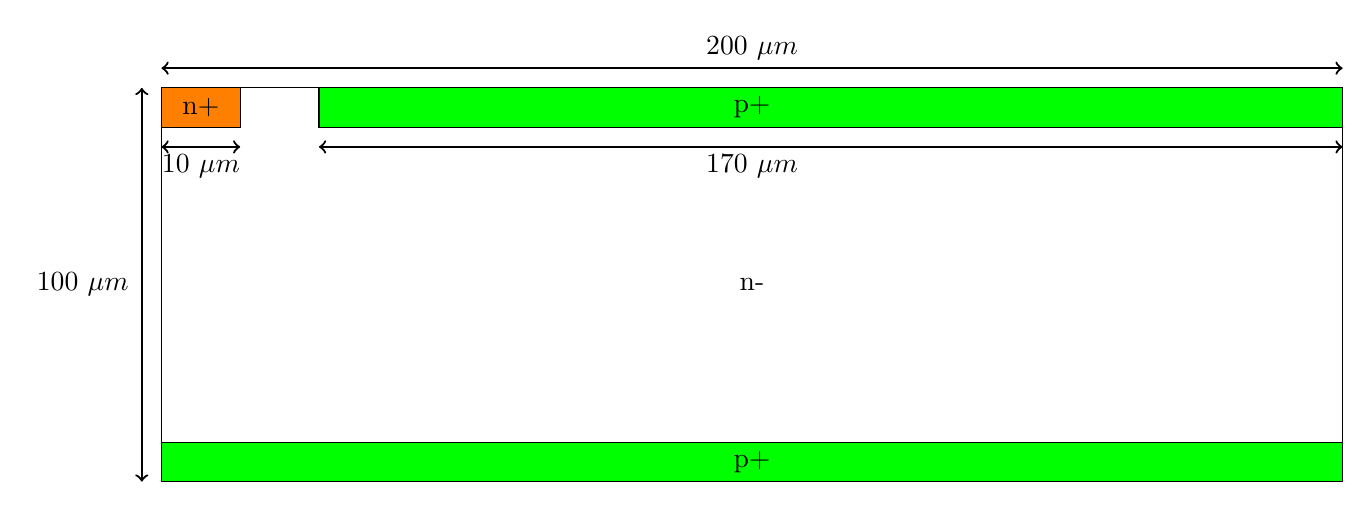
\begin{tikzpicture}
\def \thickness {5}
\def \width {15}
\draw [thick, <->] (-0.25,\thickness) -- (-0.25,0);
\draw [thick, <->] (0,\thickness+0.25) -- (\width,\thickness+0.25);
\draw [thick, <->] (2,\thickness-0.75) -- (\width,\thickness-0.75);
\node at (-1,0.5*\thickness) {100 $\mu m$};
\node at (0.5*\width,\thickness+0.5) {200 $\mu m$};
\node at (0.5*\width,\thickness-1) {170 $\mu m$};
\draw (0,0) rectangle (\width,\thickness);
\draw[fill=orange] (0,\thickness) rectangle (1,\thickness-0.5);
\draw [thick, <->] (0,\thickness-0.75) -- (1,\thickness-0.75);
\node at (0.5,\thickness-0.25) {n+};
\node at (0.5,\thickness-1) {10 $\mu m$};
\draw[fill=green] (2,\thickness-0.5) rectangle (\width,\thickness);
\node at (0.5*\width,\thickness-0.25) {p+};	
\draw[fill=green] (0,0) rectangle (\width,0.5);
\node at (0.5*\width,0.25) {p+};	
\node at (0.5*\width,0.5*\thickness) {n-};
\end{tikzpicture}
\caption{Input structure (SDD)}
\label{fig:SDD}
\end{figure}

\begin{figure}[h!]
     \centering
        \includegraphics[width=\textwidth]{equilibrium_potential_2d.png}
         \caption{Potential contour plot showing potential variation near the junction}
         \label{fig:pot_2d}
     \end{figure}

\begin{figure}[h!]
     \centering
        \includegraphics[width=\textwidth]{net_charge_equilibrium_2d.png}
         \caption{Accumulation of electrons producing negative charge near n+ region}
         \label{fig:pot_2d}
     \end{figure}

\subsection{Equilibrium potential and carrier density(1-D semiconductor p-n junction)}
Similarly, a $p+-n-n$ structure shown in \ref{fig:PIN} is solved here with similar doping profile. 
For an abrupt $p+-n$ junction \cite{bart}, depletion width is given by 
\begin{align*}
W_{dep} = \sqrt{\frac{2\epsilon_{Si} V_{bi}}{q N}} 
\end{align*}
where $N$ is the doping of lightly doped region.
For $N=10^{12}$, this is about $25 \mu m$. This is seen in the solved structure (see \ref{fig:pot_2d}) from $x=5 \mu m$ to about $x=30 \mu m$.

So, depletion width here should be about $25 \mu m$.

Built-in potential is given by 
\begin{align*}
V_{bi} \approx k_B T\ ln\left(\frac{N_A N_D}{n_i^2}\right)
\end{align*}

By above formula,it should be around 0.6 V for $p+-n$ which is seen in \ref{fig:pot_1d} at $x=10 \mu m$.

\begin{figure}[h!]
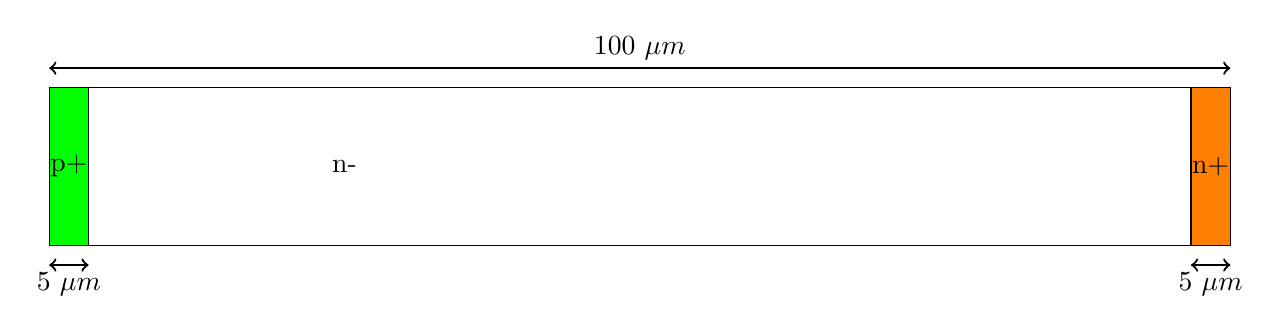
\begin{tikzpicture}
\def \thickness {2}
\def \width {15}
\draw [thick, <->] (0,\thickness+0.25) -- (\width,\thickness+0.25);
\draw [thick, <->] (0,-0.25) -- (0.5,-0.25);
\draw [thick, <->] (\width-0.5,-0.25) -- (\width,-0.25);
\node at (\width-0.25,-0.5) {5 $\mu m$};
\node at (0.25,-0.5) {5 $\mu m$};
\node at (0.5*\width,\thickness+0.5) {100 $\mu m$};
\draw (0,0) rectangle (\width,\thickness);
\draw[fill=green] (0,0) rectangle (0.5,\thickness);
\node at (0.25,0.5*\thickness) {p+};
\draw[fill=orange] (\width-0.5,0) rectangle (\width,\thickness);
\node at (\width-0.25,0.5*\thickness) {n+};
\node at (0.25*\width,0.5*\thickness) {n-};
\end{tikzpicture}
\caption{PIN diode}
\label{fig:PIN}
\end{figure}

\begin{figure}[h!]
     \centering
        \includegraphics[width=0.8\textwidth]{equilibrium_Potential_1d.png}
         \caption{Equilibrium Potential}
         \label{fig:pot_1d}	
     \end{figure}
     
\begin{figure}[h!]
     \centering
        \includegraphics[width=0.8\textwidth]{total_carriers_equilibrium.png}
         \caption{Carrier depletion near the $p+-n$ junction}
         \label{fig:car_1d}	
     \end{figure}     

\subsection{Potential and current density in a biased p-n junction}
In reverse bias, a potential barrier exists which blocks the flow of current while in forward bias, barrier lowers and large current flows. These features are visible in the following results.
 
\begin{figure}[h!]
     \centering
        \includegraphics[width=0.8\textwidth]{comparision_pin_fb.png}
         \caption{Potential barrier lowered in forward bias (compare with \ref{fig:pot_1d})}
         \label{fig:pot_fb}
     \end{figure}
     
\begin{figure}[h!]
     \centering
        \includegraphics[width=0.8\textwidth]{comparision_pin_rb.png}
         \caption{Potential barrier increased in reverse bias (compare with \ref{fig:pot_1d})}
         \label{fig:pot_fb}
     \end{figure}     

Current density for an ideal pn-junction diode \cite{bart} can be approximated by :
\begin{align*}
J = J_0 (e^{qV/k_BT}-1) 
\end{align*}


Current density for \ref{fig:PIN} is calculated.

\begin{figure}[h!]
     \centering
        \includegraphics[width=0.8\textwidth]{jv_diode_linear.png}
         \caption{Current density (Linear scale)}
         \label{fig:jv}
     \end{figure}

\begin{figure}[h!]
     \centering
        \includegraphics[width=0.8\textwidth]{jv_diode_log.png}
         \caption{Current density (Logarithmic scale) (compare with \ref{fig:jv_bart})}
		 \label{fig:jvl}     
     \end{figure}

\begin{figure}[h!]
     \centering
        \includegraphics[width=0.8\textwidth]{bart.png}
         \caption{Image taken from \cite{bart}}
		 \label{fig:jv_bart}     
     \end{figure}

In forward bias, current becomes very high when $V>=V_{bi}$. Here, $V_{bi} = 0.6\ V$. In reverse bias, very low current flows (see  \ref{fig:jv}). Also, exponential relationship can be seen as J-V plot is linear in logarithmic scale in forward bias as seen in \ref{fig:jvl}.


\clearpage
\bibliographystyle{unsrt}
\bibliography{ref}

\end{document}
